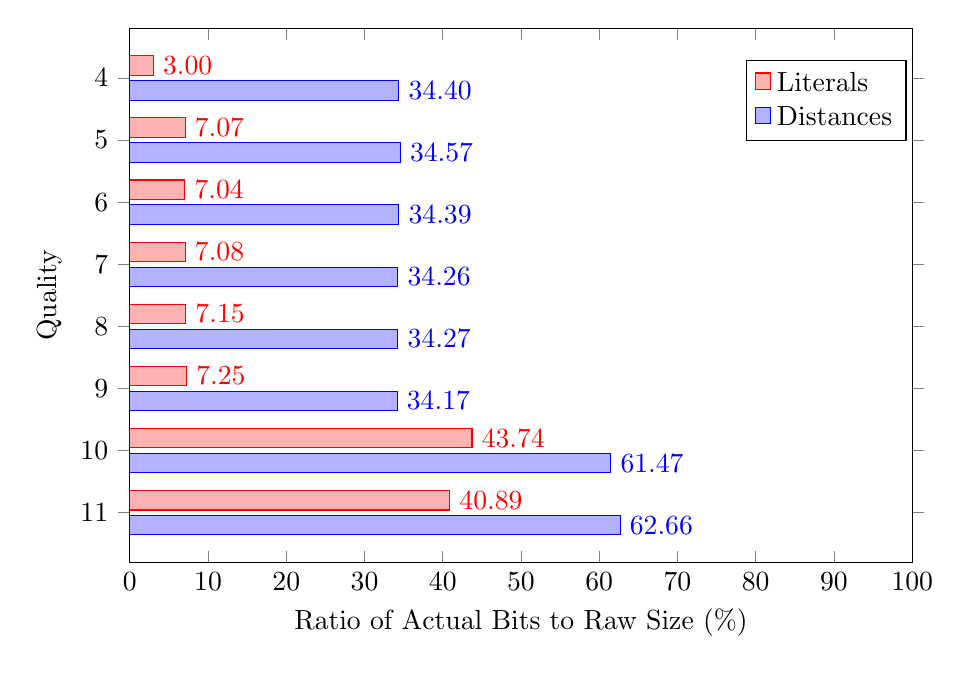
\begin{tikzpicture}
\begin{axis}[
	width = 0.95\textwidth,
	height = 1.15*\axisdefaultheight,
	xbar,
	xmin = 0,
	xmax = 100,
	xtick = {0, 10, 20, 30, 40, 50, 60, 70, 80, 90, 100},
	y dir = reverse,
	ytick = data,
	bar width = 7pt,
	scaled ticks = false,
	enlarge x limits = {abs = 0},
	enlarge y limits = {abs = 0.8},
	reverse legend,
	legend cell align = {left},
	legend style = {
		at = {(0.89, 0.94)},
		anchor = north
	},
	legend image code/.code = {
		\draw[#1] (0cm, -0.075cm) rectangle (0.2cm, 0.135cm);
	},
	nodes near coords,
	nodes near coords align = {horizontal},
	nodes near coords style = {/pgf/number format/.cd, fixed zerofill, precision = 2},
	xlabel = Ratio of Actual Bits to Raw Size (\%),
	ylabel = Quality
]
\legend{
	Distances,
	Literals
}
\addplot coordinates {
	(34.40, 4)
	(34.57, 5)
	(34.39, 6)
	(34.26, 7)
	(34.27, 8)
	(34.17, 9)
	(61.47, 10)
	(62.66, 11)
};
\addplot coordinates {
	(3.00, 4)
	(7.07, 5)
	(7.04, 6)
	(7.08, 7)
	(7.15, 8)
	(7.25, 9)
	(43.74, 10)
	(40.89, 11)
};
\end{axis}
\end{tikzpicture}